\chapter{v2 robustness study}
\label{chap:robustness}

The synthetic numbers of \cref{chap:results} all assume that the
deployment distribution matches the training distribution. In
practice, a beacon will see varying noise conditions and anomaly
shapes that the templates do not capture exactly. This chapter
quantifies how gracefully each architecture degrades when the
deployment data is forced out of distribution along two controlled
axes.

\section{Protocol}
\label{sec:rob-protocol}

The robustness script \texttt{architectures/robustness\_test.py} calls
the v2 generator with two distortion knobs.
\begin{enumerate}[leftmargin=*, itemsep=0.2em]
    \item \textbf{Background-noise sweep.} The AR(1) innovation
    standard deviation $\sigma_\varepsilon$ is multiplied by
    $m_{\text{noise}} \in [1, 3]$, ten evenly-spaced values. The
    marginal HF noise standard deviation $\sigma_r$ scales by the same
    factor. The anomaly amplitudes are \emph{not} rescaled: with v2's
    absolute amplitudes, the SNR drops naturally as the noise grows
    (in contrast to v1, where the SNR was held constant by rescaling
    amplitudes).
    \item \textbf{Anomaly-shape-deformation sweep.} The
    deformation-variance parameter $\nu$ of the template generator
    (\cref{sec:v1-deformation}) is multiplied by $m_{\text{deform}}
    \in [1, 8]$, ten evenly-spaced values. The noise multiplier is
    held at $1$.
\end{enumerate}

Each generated test dataset contains $50$ events, evaluated with the
event-level protocol of \cref{sec:event-eval}. The metric reported is
the macro F1 across the three anomaly classes.

\section{Results}
\label{sec:rob-results}

\begin{figure}[H]
    \centering
    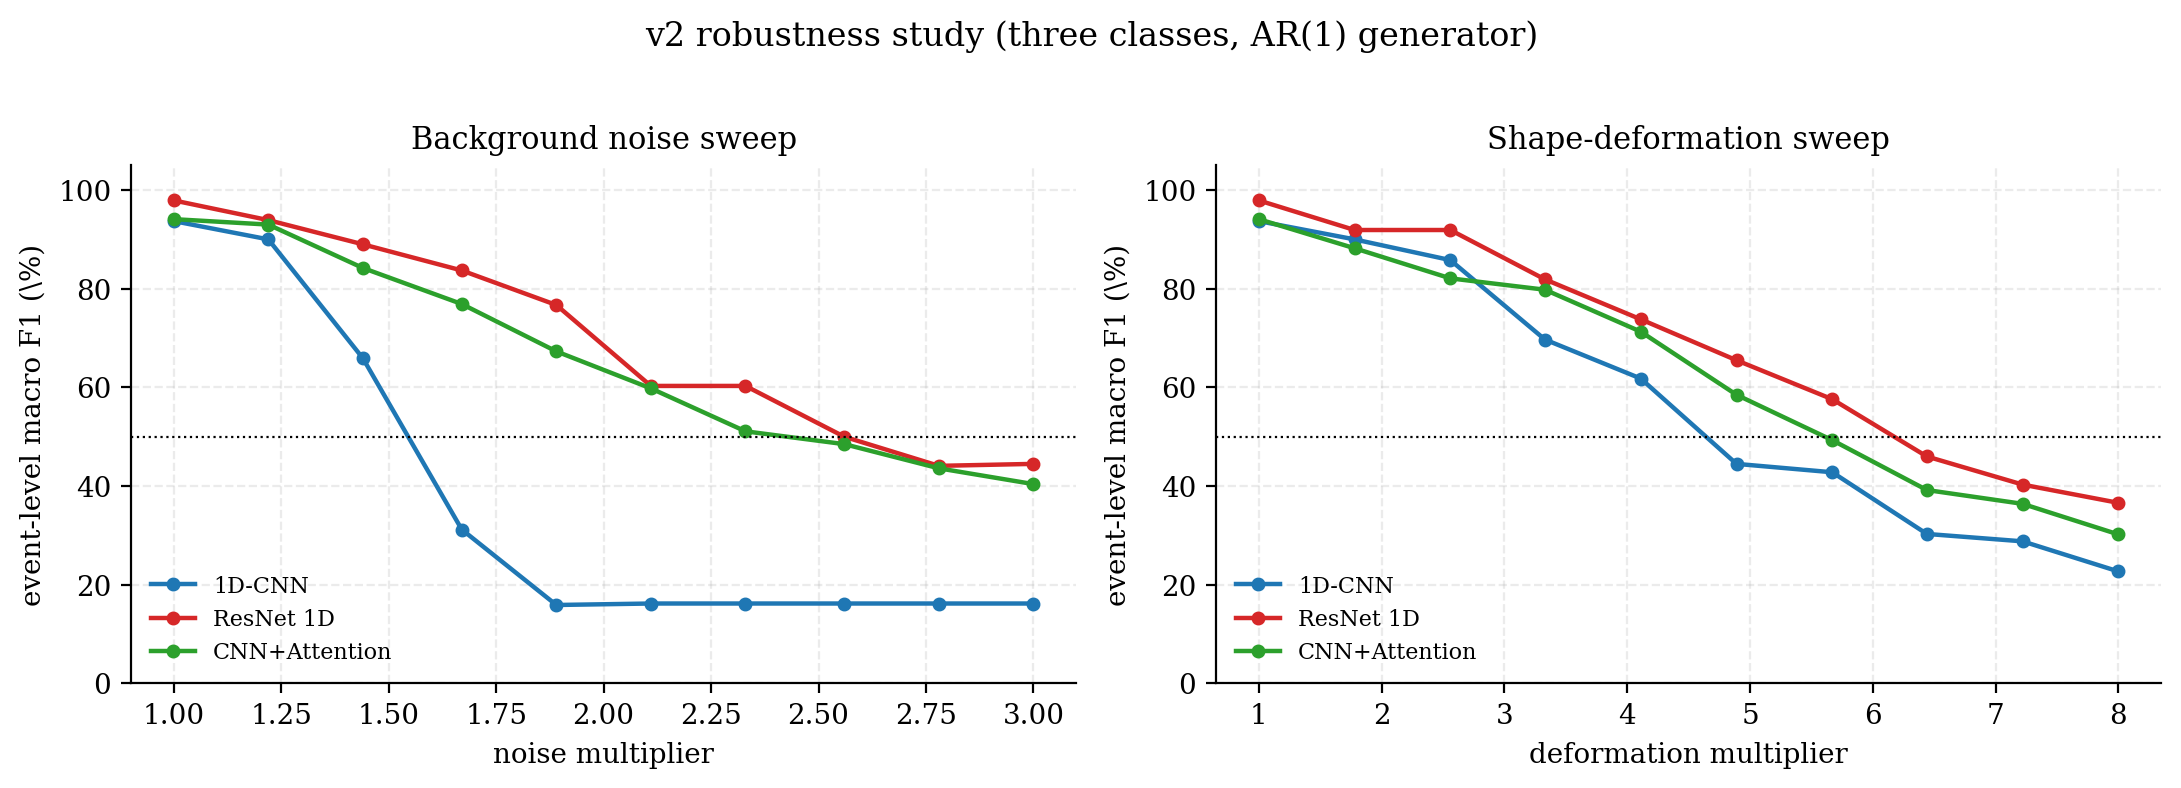
\includegraphics[width=\linewidth]{figures/v2_robustness}
    \caption{v2 robustness curves. \textbf{Left}: event-level macro F1
    as a function of the background-noise multiplier. \textbf{Right}:
    macro F1 as a function of the anomaly-shape deformation
    multiplier. The dotted line marks the $50\%$ threshold.}
    \label{fig:v2-robustness}
\end{figure}

\paragraph{Background-noise sweep.}
\begin{itemize}[leftmargin=*, itemsep=0.2em]
    \item The \textbf{1D-CNN} F1 drops below $50\%$ already at
    $m_{\text{noise}} \approx 1.7$ and continues to collapse to
    $\sim 16\%$ for the rest of the sweep --- the same kind of
    single-class collapse already visible in v1
    (\cref{fig:v1-robustness}, left).
    \item The \textbf{ResNet} is the most robust on this axis: F1
    stays above $50\%$ until $m_{\text{noise}} \approx 2.8$ and still
    sits at $\sim 44\%$ at the end of the sweep ($m_{\text{noise}} =
    3$, three times the training noise).
    \item The \textbf{CNN+Attention} falls between the two: it
    crosses $50\%$ at $m_{\text{noise}} \approx 2.6$ and finishes at
    $\sim 40\%$ --- close to the ResNet but distinguishably below it.
\end{itemize}

\paragraph{Shape-deformation sweep.}
\begin{itemize}[leftmargin=*, itemsep=0.2em]
    \item The \textbf{1D-CNN} drops below $50\%$ at $m_{\text{deform}}
    \approx 4.9$.
    \item The \textbf{ResNet} stays above $50\%$ until $m_{\text{deform}}
    \approx 6.4$, the \textbf{CNN+Attention} until $m_{\text{deform}}
    \approx 5.7$.
    \item All three models degrade smoothly --- no abrupt
    single-class collapse on this axis.
\end{itemize}

\section{v1 vs v2 robustness in one figure}
\label{sec:rob-v1-v2}

\Cref{fig:v1-vs-v2-robustness} puts the two iterations side by side
for direct comparison.

\begin{figure}[H]
    \centering
    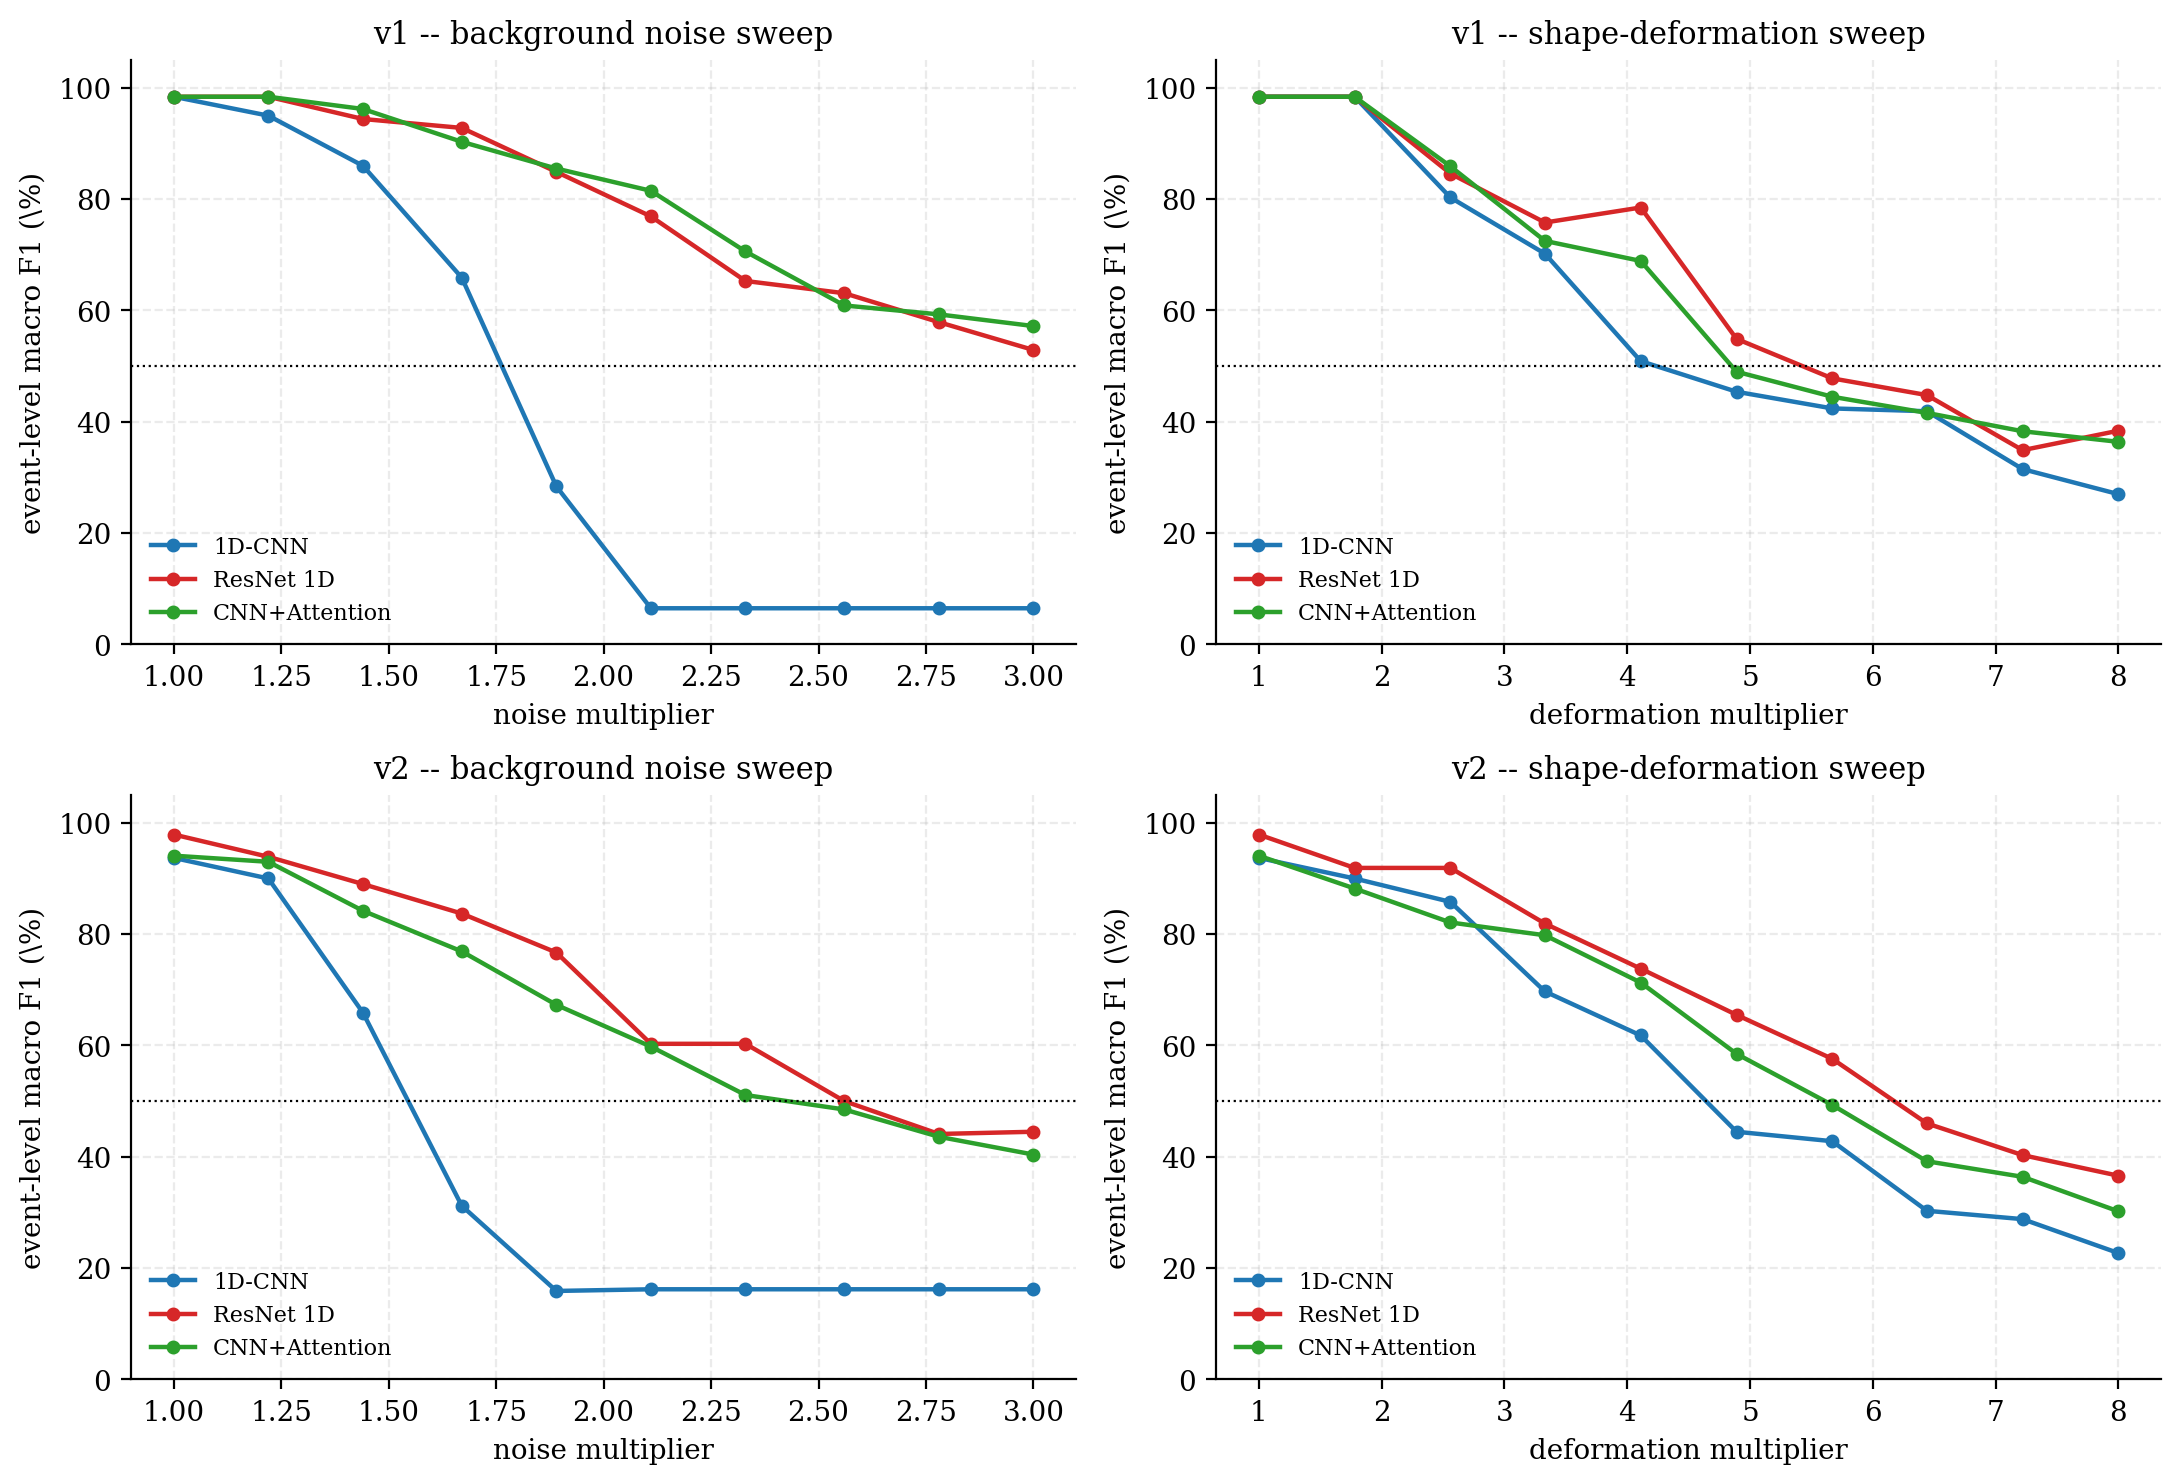
\includegraphics[width=\linewidth]{figures/v1_vs_v2_robustness}
    \caption{Robustness curves of v1 (top row) and v2 (bottom row) on
    the same axes. The vertical position of the curves is not directly
    comparable between the two iterations --- v1 reports macro F1 over
    six classes, v2 over three --- but the qualitative behaviour is.
    The collapse of the 1D-CNN at high noise is much more brutal in
    v1 (drop to $\sim 7\%$) than in v2 (gentler drop to $\sim 4\%$
    by the end of the sweep), and the residual / attention models are
    qualitatively similar in both iterations.}
    \label{fig:v1-vs-v2-robustness}
\end{figure}

\section{Discussion}
\label{sec:rob-discuss}

\paragraph{Residual connections are the single biggest win on
robustness.} The gap between the baseline 1D-CNN and the ResNet on the
noise axis is enormous in both iterations. The two architectures share
the same trunk depth and the same classifier head; the differences are
(i) residual connections and (ii) GroupNorm instead of BatchNorm. Both
ingredients point in the same direction --- a network whose features
survive a small distribution shift in the input is structurally
important for an operational beacon.

\paragraph{Self-attention does not buy extra robustness here.} The
CNN+Attention model sits between the 1D-CNN and the ResNet on both
axes --- close to the ResNet but distinguishably below it. The
Transformer encoder layers add capacity for long-range reasoning, but
the window in this problem is short ($512$ samples) and the v2
anomalies rarely extend past $\sim 800$ samples, so attention does
not have much extra context to exploit. On a much longer window ---
say a $24$-hour window with several events of interest --- we would
expect the attention model to pull ahead.

\paragraph{Why the v2 noise robustness curve is gentler than v1.} The
v1 robustness sweep held the absolute SNR constant by dividing the
anomaly amplitude by the noise multiplier; the v2 sweep does not.
That makes the v2 sweep a slightly easier test --- the noise grows
but the anomaly amplitude stays at the v2 absolute range $[15, 40]$
counts. The fact that the 1D-CNN \emph{still} collapses below $50\%$
F1 by $m_{\text{noise}} \approx 1.7$ confirms that the BatchNorm-based
1D-CNN is intrinsically fragile to noise growth.

\paragraph{Operational implications.} A beacon that runs across
seasons easily sees a $\times 1.5$ multiplier on the high-frequency
noise. The robustness curves argue that the residual or attention
architecture is the only viable choice if the system has to keep
functioning across seasons without retraining.
